\normaltrue
\correctionfalse

%\UPSTIidClasse{11} % 11 sup, 12 spé
%\newcommand{\UPSTIidClasse}{12}

\exer{Mouvement RR  $\star$ \label{CIN:01:B2:13:PTSI:04:02}}
\setcounter{question}{0}\UPSTIcompetence{B2-13}
\index{Compétence B2-13-PTSI}
\index{Mécanisme à 2 rotations}
\ifcorrection
\else
\marginnote{\textbf{Pas de corrigé pour cet exercice.}}
\fi

\ifprof
\else
Soit le mécanisme suivant. 
\begin{marginfigure}
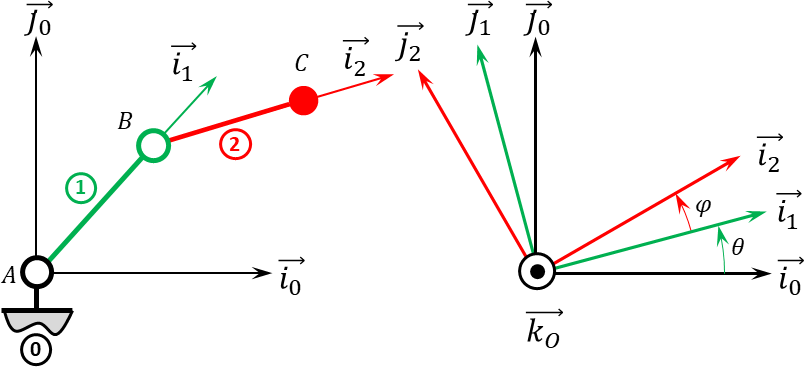
\includegraphics[width=\linewidth]{04_RR_01}
\end{marginfigure}
\fi

\question{Réaliser le paramétrage du mécanisme.}
\ifprof ~\\
\else

\fi



\ifprof
\else
\footnotesize

\normalsize
\marginnote{Corrigé voir \ref{CIN:01:B2:13:PTSI:04:02}.}

\fi